\documentclass[14pt,a4paper]{report}  %紙張設定
\usepackage{xeCJK}%中文字體模組
%\setCJKmainfont{標楷體} %設定中文字體
\setCJKmainfont{MoeStandardKai.ttf}
%\newfontfamily\sectionef{Times New Roman}%設定英文字體
\newfontfamily\sectionef{Nimbus Roman}
\usepackage{enumerate}
\usepackage{amsmath,amssymb}%數學公式、符號
\usepackage{amsfonts} %數學簍空的英文字
\usepackage{graphicx, subfigure}%圖形
\usepackage{fontawesome5} %引用icon
\usepackage{type1cm} %調整字體絕對大小
\usepackage{textpos} %設定文字絕對位置
\usepackage[top=2.5truecm,bottom=2.5truecm,
left=3truecm,right=2.5truecm]{geometry}
\usepackage{titlesec} %目錄標題設定模組
\usepackage{titletoc} %目錄內容設定模組
\usepackage{textcomp} %表格設定模組
\usepackage{multirow} %合併行
%\usepackage{multicol} %合併欄
\usepackage{CJK} %中文模組
\usepackage{CJKnumb} %中文數字模組
\usepackage{wallpaper} %浮水印
\usepackage{listings} %引用程式碼
\usepackage{hyperref} %引用url連結
\usepackage{setspace}
\usepackage{lscape}%設定橫式
\lstset{language=Python, %設定語言
		basicstyle=\fontsize{10pt}{2pt}\selectfont, %設定程式內文字體大小
		frame=lines,	%設定程式框架為線
}
%\usepackage{subcaption}%副圖標
\graphicspath{{./../images/}} %圖片預設讀取路徑
\usepackage{indentfirst} %設定開頭縮排模組
\renewcommand{\figurename}{\Large 圖.} %更改圖片標題名稱
\renewcommand{\tablename}{\Large 表.}
\renewcommand{\lstlistingname}{\Large 程式.} %設定程式標示名稱
\hoffset=-5mm %調整左右邊界
\voffset=-8mm %調整上下邊界
\setlength{\parindent}{3em}%設定首行行距縮排
\usepackage{appendix} %附錄
\usepackage{diagbox}%引用表格
\usepackage{multirow}%表格置中
%\usepackage{number line}
%=------------------更改標題內容----------------------=%
\titleformat{\chapter}[hang]{\center\sectionef\fontsize{20pt}{1pt}\bfseries}{\LARGE 第\CJKnumber{\thechapter}章}{1em}{}[]
\titleformat{\section}[hang]{\sectionef\fontsize{18pt}{2.5pt}\bfseries}{{\thesection}}{0.5em}{}[]
\titleformat{\subsection}[hang]{\sectionef\fontsize{18pt}{2.5pt}\bfseries}{{\thesubsection}}{1em}{}[]
%=------------------更改目錄內容-----------------------=%
\titlecontents{chapter}[11mm]{}{\sectionef\fontsize{18pt}{2.5pt}\bfseries\makebox[3.5em][l]
{第\CJKnumber{\thecontentslabel}章}}{}{\titlerule*[0.7pc]{.}\contentspage}
\titlecontents{section}[18mm]{}{\sectionef\LARGE\makebox[1.5em][l]
{\thecontentslabel}}{}{\titlerule*[0.7pc]{.}\contentspage}
\titlecontents{subsection}[4em]{}{\sectionef\Large\makebox[2.5em][l]{{\thecontentslabel}}}{}{\titlerule*[0.7pc]{.}\contentspage}
%=----------------------章節間距----------------------=%
\titlespacing*{\chapter} {0pt}{0pt}{18pt}
\titlespacing*{\section} {0pt}{12pt}{6pt}
\titlespacing*{\subsection} {0pt}{6pt}{6pt}
%=----------------------標題-------------------------=%             
\begin{document} %文件
\sectionef %設定英文字體啟用
\vspace{12em}
\begin{titlepage}%開頭
\begin{center}   %標題  
\makebox[1.5\width][s] %[s] 代表 Stretch the interword space in text across the entire width
{\fontsize{24pt}{2.5pt}國立虎尾科技大學}\\[18pt]
\makebox[1.5\width][s]
{\fontsize{24pt}{2.5pt}機械設計工程系}\\[18pt]
\sectionef\fontsize{24pt}{1em}\selectfont\textbf
{
\vspace{0.5em}
cd2023 2b-pj2bg7分組報告}\\[18pt]
%設定文字盒子 [方框寬度的1.5倍寬][對其方式為文字平均分分布於方框中]\\距離下方18pt
\vspace{1em} %下移
\fontsize{30pt}{1pt}\selectfont\textbf{網際足球場景設計}\\
\vspace{1em}
\sectionef\fontsize{30pt}{1em}\selectfont\textbf
{
\vspace{0.5em}
Web-based Football Scene Design}
 \vspace{2em}
%=---------------------參與人員-----------------------=%             
\end{center}
\begin{flushleft}
\begin{LARGE}

\hspace{32mm}\makebox[5cm][s]
{指導教授:\quad 嚴\quad 家\quad 銘\quad 老\quad 師}\\[6pt]
\hspace{32mm}\makebox[5cm][s]
{班\qquad 級:\quad 四\quad 設\quad 二\quad 乙}\\[6pt]
\hspace{32mm}\makebox[5cm][s]
{學\qquad 生:\quad 陳\quad 冠\quad 佑\quad(41023219)}
\\[6pt]
\hspace{32mm}\makebox[5cm][s]
{\hspace{36.5mm}陳\quad 冠\quad 翰\quad(41023221)}\\[6pt]
\hspace{32mm}\makebox[5cm][s]
{\hspace{36.5mm}陳\quad 奕\quad 倫\quad(41023222)}\\[6pt]
\hspace{32mm}\makebox[5cm][s]
{\hspace{36.5mm}陳\quad 瑨\quad 維\quad(41023228)}\\[6pt]
\hspace{32mm}\makebox[5cm][s]

%設定文字盒子[寬度為5cm][對其方式為文字平均分分布於方框中]空白距離{36.5mm}\空白1em
\end{LARGE}
\end{flushleft}
\vspace{6em}
\fontsize{18pt}{2pt}\selectfont\centerline{\makebox[\width][s]
{中華民國\hspace{3em} 
112 \quad 年\quad 5\quad 月}}
\end{titlepage}
\newpage



%=------------------------摘要-----------------------=%
\renewcommand{\baselinestretch}{1.5} %設定行距
\pagenumbering{roman} %設定頁數為羅馬數字
\clearpage  %設定頁數開始編譯
\sectionef
\addcontentsline{toc}{chapter}{摘~~~要} %將摘要加入目錄
\begin{center}
\LARGE\textbf{摘~~要}\\
\end{center}
\begin{flushleft}
\fontsize{14pt}{20pt}\sectionef\hspace{12pt}\quad 由於矩陣計算、自動求導技術、開源開發環境、多核GPU運算硬體等這四大發展趨勢,促使AI領域快速發展,藉由這樣的契機,將實體機電系統透過虛擬化訓練提高訓練效率,再將訓練完的模型應用到實體上。\\[12pt]

\fontsize{14pt}{20pt}\sectionef\hspace{12pt}\quad 此專題是運用實體冰球對打機,將其導入CoppeliaSim模擬環境並給予對應設置,將其機電系統簡化並運用Open AI Gym進行訓練,找到適合此系統的演算法後,再到CoppeliaSim模擬環境中進行測試演算法在實際運用上的可行性。並嘗試透過架設伺服器將CoppeliaSim影像串流到網頁供使用者觀看或操控。\\[12pt]

\end{flushleft}
\begin{center}
\fontsize{14pt}{20pt}\selectfont 關鍵字: 類神經網路、強化學習、\sectionef CoppeliaSim、OpenAI Gym
\end{center}
\newpage
%=--------------------Abstract----------------------=%
\renewcommand{\baselinestretch}{1.5} %設定行距
\addcontentsline{toc}{chapter}{Abstract} %將摘要加入目錄
\begin{center}
\LARGE\textbf\sectionef{Abstract}\\
\begin{flushleft}
\fontsize{14pt}{16pt}\sectionef\hspace{12pt}\quad Due to the four major development trends of multidimensional arrays  computing, automatic differentiation, open source development environment, and multi-core GPUs computing hardware. The rapid development of the AI field has been promoted. In view of this development, the physical mechatronic systems can gain machine learning efficiency through their simulated virtual system training process. And afterwards to apply the trained model into real mechatronic systems.\\[12pt]

\fontsize{14pt}{16pt}\sectionef\hspace{12pt}\quad This project is to use the physical air hockey to play machine, introduce it into the CoppeliaSim simulation environment and give the corresponding settings, simplify its electromechanical system and use Open AI Gym for training, find an algorithm suitable for this system, and then perform it in the CoppeliaSim simulation environment Feasibility of testing algorithm in practical application. And try to stream CoppeliaSim images to web pages for users to watch or manipulate by setting up a server.\\
\end{flushleft}
\begin{center}
\fontsize{14pt}{16pt}\selectfont\sectionef Keyword:  nerual network、reinforcement learning、 CoppeliaSim、OpenAI Gym
\end{center}
\newpage
%=------------------------誌謝----------------------=%
\addcontentsline{toc}{chapter}{誌~~~謝}
\centerline\LARGE\textbf{誌~~謝}\\
\begin{flushleft}
\fontsize{14pt}{2.5pt}\hspace{12pt}\quad 在此鄭重感謝製作以及協助本分組報告完成的所有人員,首先向嚴家銘老師致謝,他解決我們的各種提問,甚至從來沒有不耐煩,總是貼心為我們找出最佳解答。再來是第 12 組的 41023251 鄭立揚同學,他給了我們全方位的支援,提供我們解決問題的建議,最後是由本分組成員同心協力才得以完成本報告,特此感謝
\end{flushleft}
\newpage
%=------------------------目錄----------------------=%
\renewcommand{\contentsname}{\centerline{\fontsize{18pt}{\baselineskip}\selectfont\textbf{目\quad 錄}}}
\tableofcontents  %目錄產生
\newpage

%=-------------------------內容----------------------=%
\chapter{前言}
\renewcommand{\baselinestretch}{10.0} %設定行距
\pagenumbering{arabic} %設定頁號阿拉伯數字
\setcounter{page}{1}  %設定頁數
\fontsize{14pt}{2.5pt}\sectionef
\section{研究動機}
機器學習與各領域結合的應用越來越廣泛,在機電系統採用強化學習是為了讓機電系統的控制達到最佳化。本專題以實體的冰球機(圖.\ref{fig.冰球機})之機電系統作為訓練模型,將實體機器轉移到虛擬環境(圖.\ref{fig.模擬冰球機})進行模擬,為了找到適合的訓練參數,因此將模型簡化(圖.\ref{fig.pong_gym})後再進行測試各種參數的優劣,透過不斷的訓練來得到一個優化過的對打系統。\\

\begin{figure}[hbt!]
\begin{center}
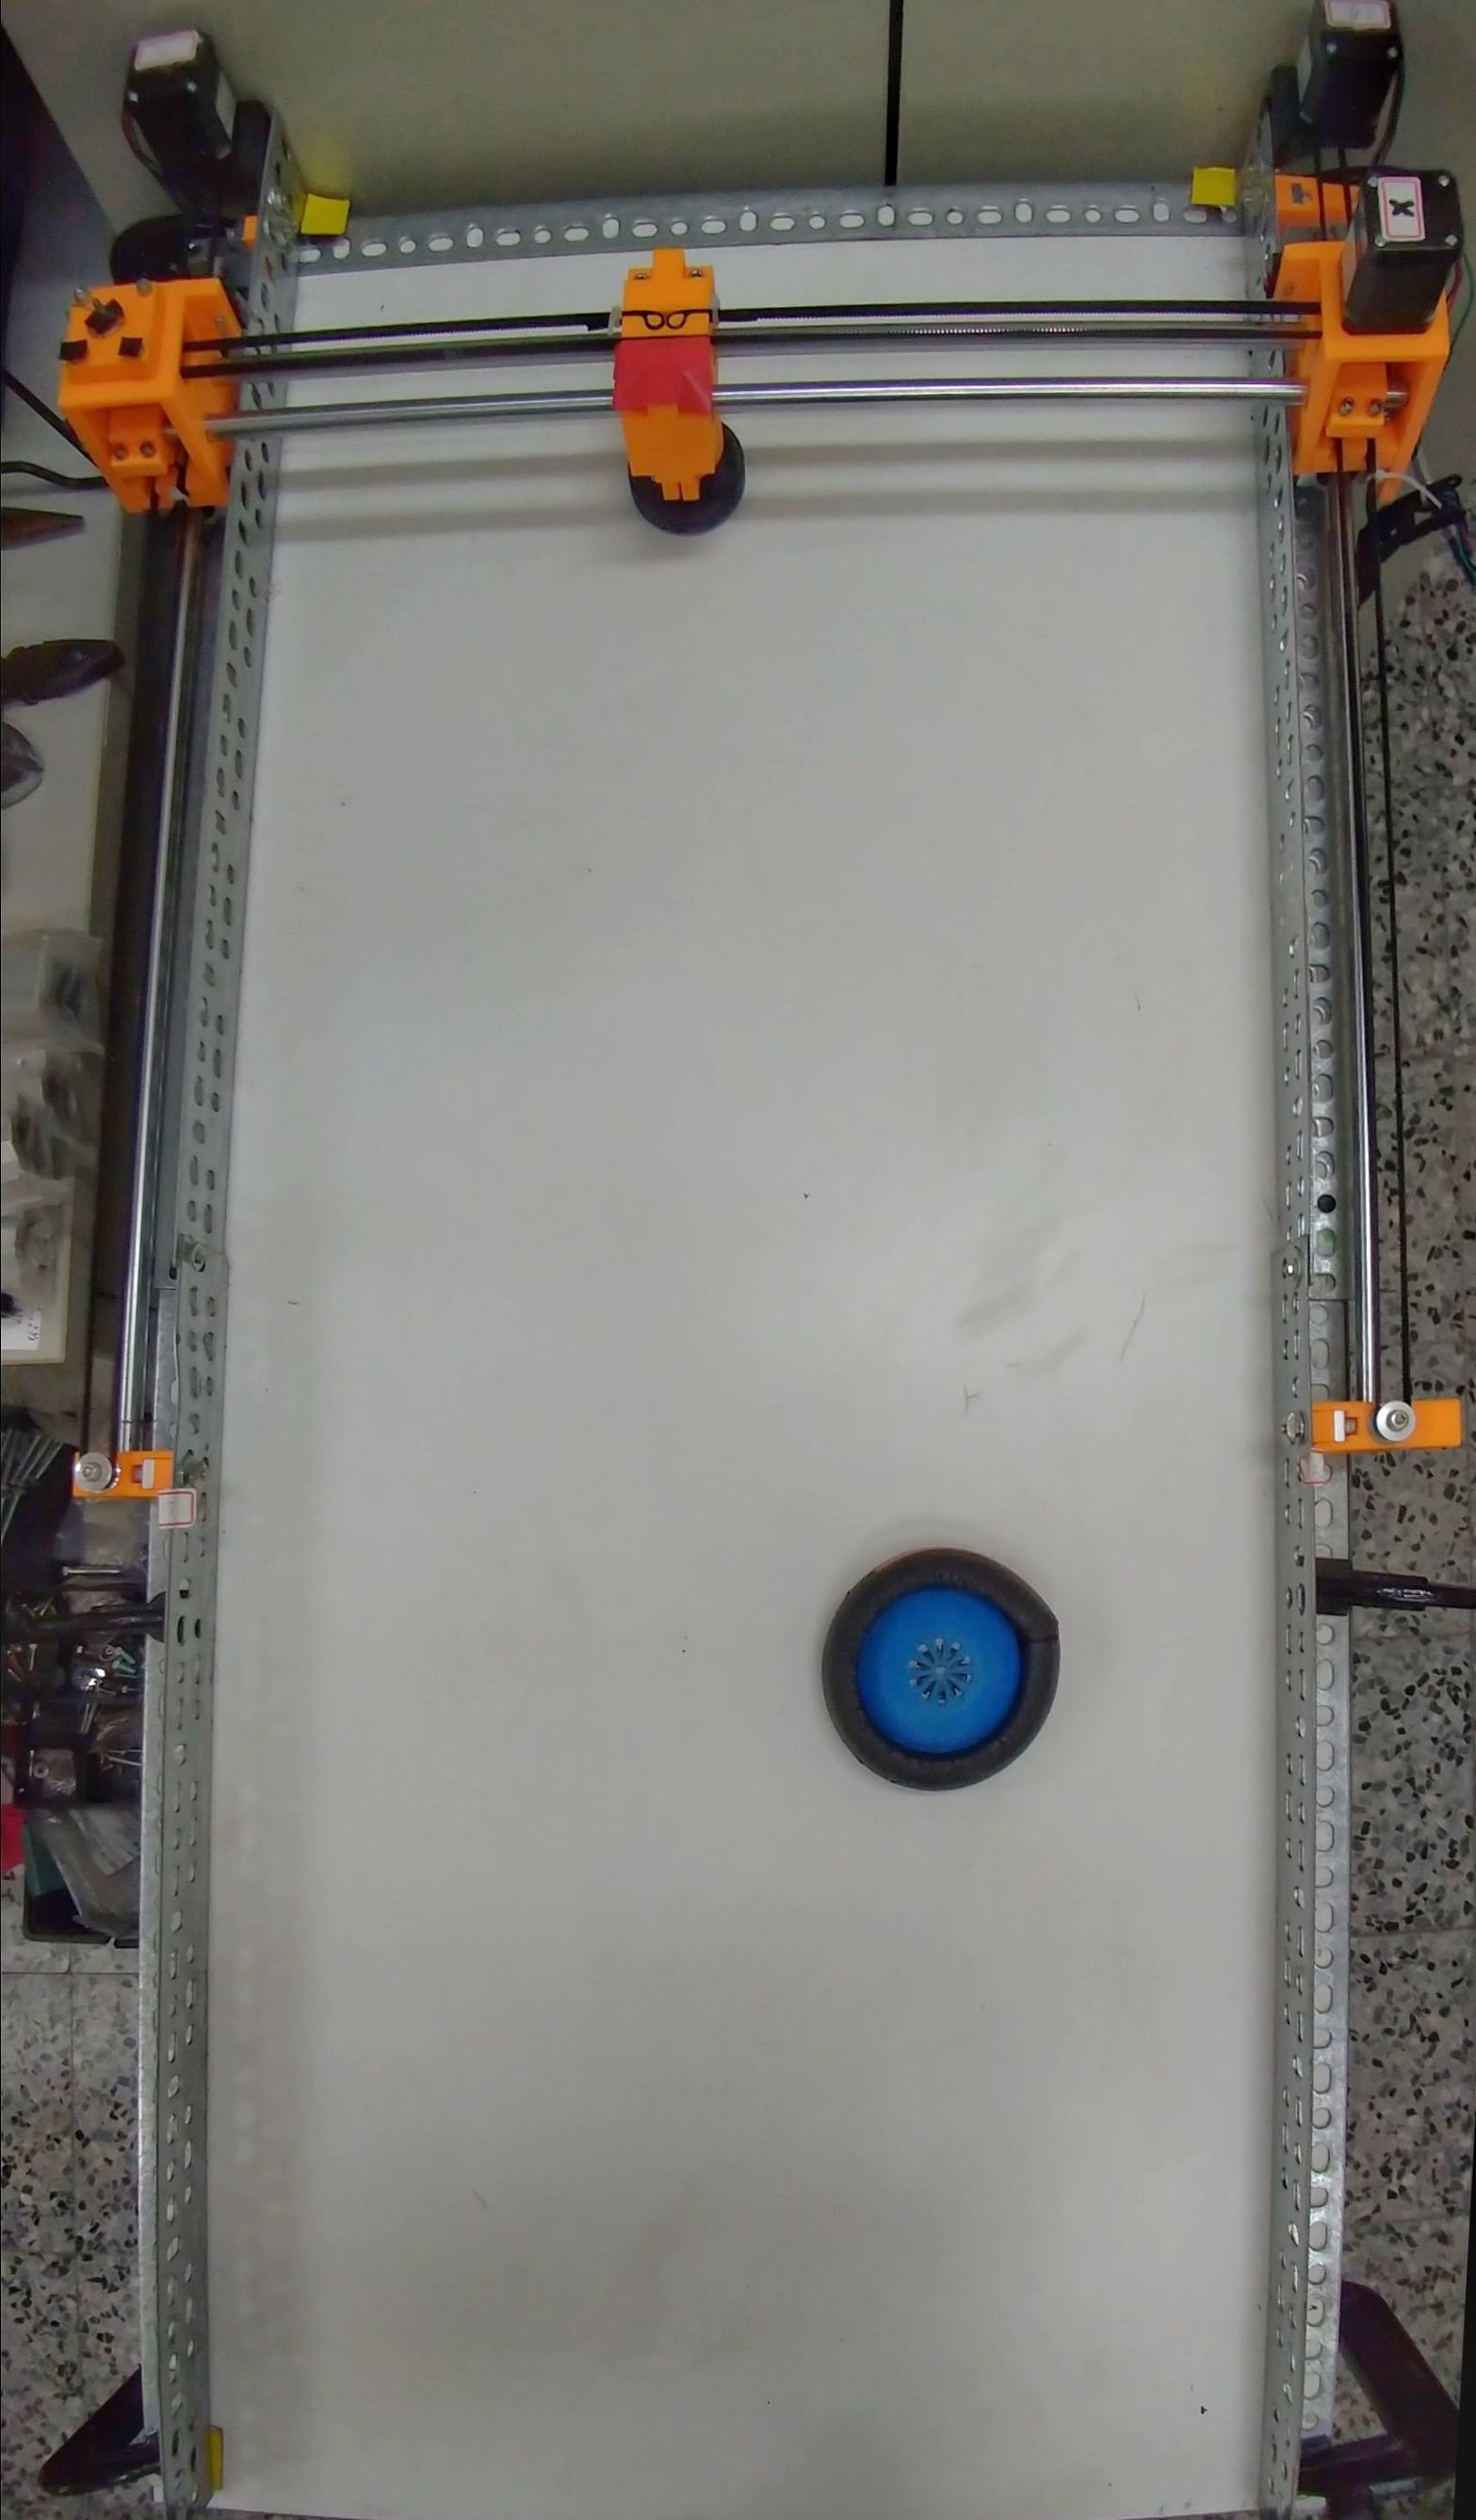
\includegraphics[angle=90,width=10cm]{冰球機}
\caption{\Large 實體的冰球機}\label{fig.冰球機}
\end{center}
\end{figure}
\begin{figure}[hbt!]
\begin{center}
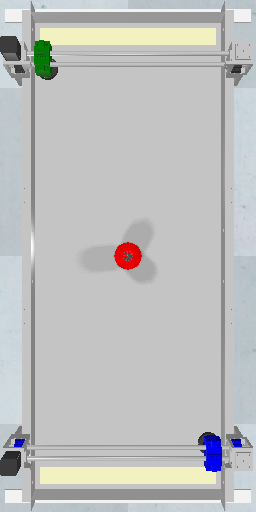
\includegraphics[angle=90,width=10cm]{origin}
\caption{\Large 虛擬環境簡化後的冰球機}\label{fig.模擬冰球機}
\end{center}
\end{figure}
\begin{figure}[hbt!]
\begin{center}
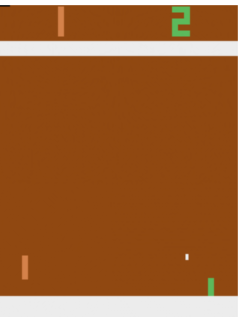
\includegraphics[height=8cm]{pong_gym}
\caption{\Large Gym的Pong game}\label{fig.pong_gym}
\end{center}
\end{figure}


\section{研究目的與方法}
本研究分三大部分,第一運用OpenAI Gym裡內建編譯的ATARI 2600遊戲Pong-v0,來作為訓練環境,加上強化學習的理論,測試不同演算法參數以訓練出最佳化的對打系統,第二將整個簡化後冰球機導入CoppilaSim模擬環境並嘗試進行虛擬訓練,成為優化的對打機電系統。第三則是嘗試透過架設伺服器與虛擬環境結合。\\
 
透過簡化實體冰球機並導入虛擬環境,進行虛擬訓練,使用Gym的Pong當作對應的2D虛擬訓練環境,測試算法和訓練效果,篩選適合的算法與參數。\\

建置CoppilaSim模擬環境,嘗試將2D訓練概念套用到3D環境進行測試,加入電腦視覺與RemoteAPI,電腦視覺抓取球與擊錘的位置,透過RemoteAPI進行遠端控制,在3D環境測試算法可確保後續套用到實體機器上的可行性。\\
 
 再透過架設伺服器與虛擬環境結合:讓虛擬環境的影像透過網伺服器串流影像供使用者遠端進行操控虛擬環境的擊錘進行打球,或是提供多人進行觀看對打影像。
\begin{figure}[hbt!]
\begin{center}
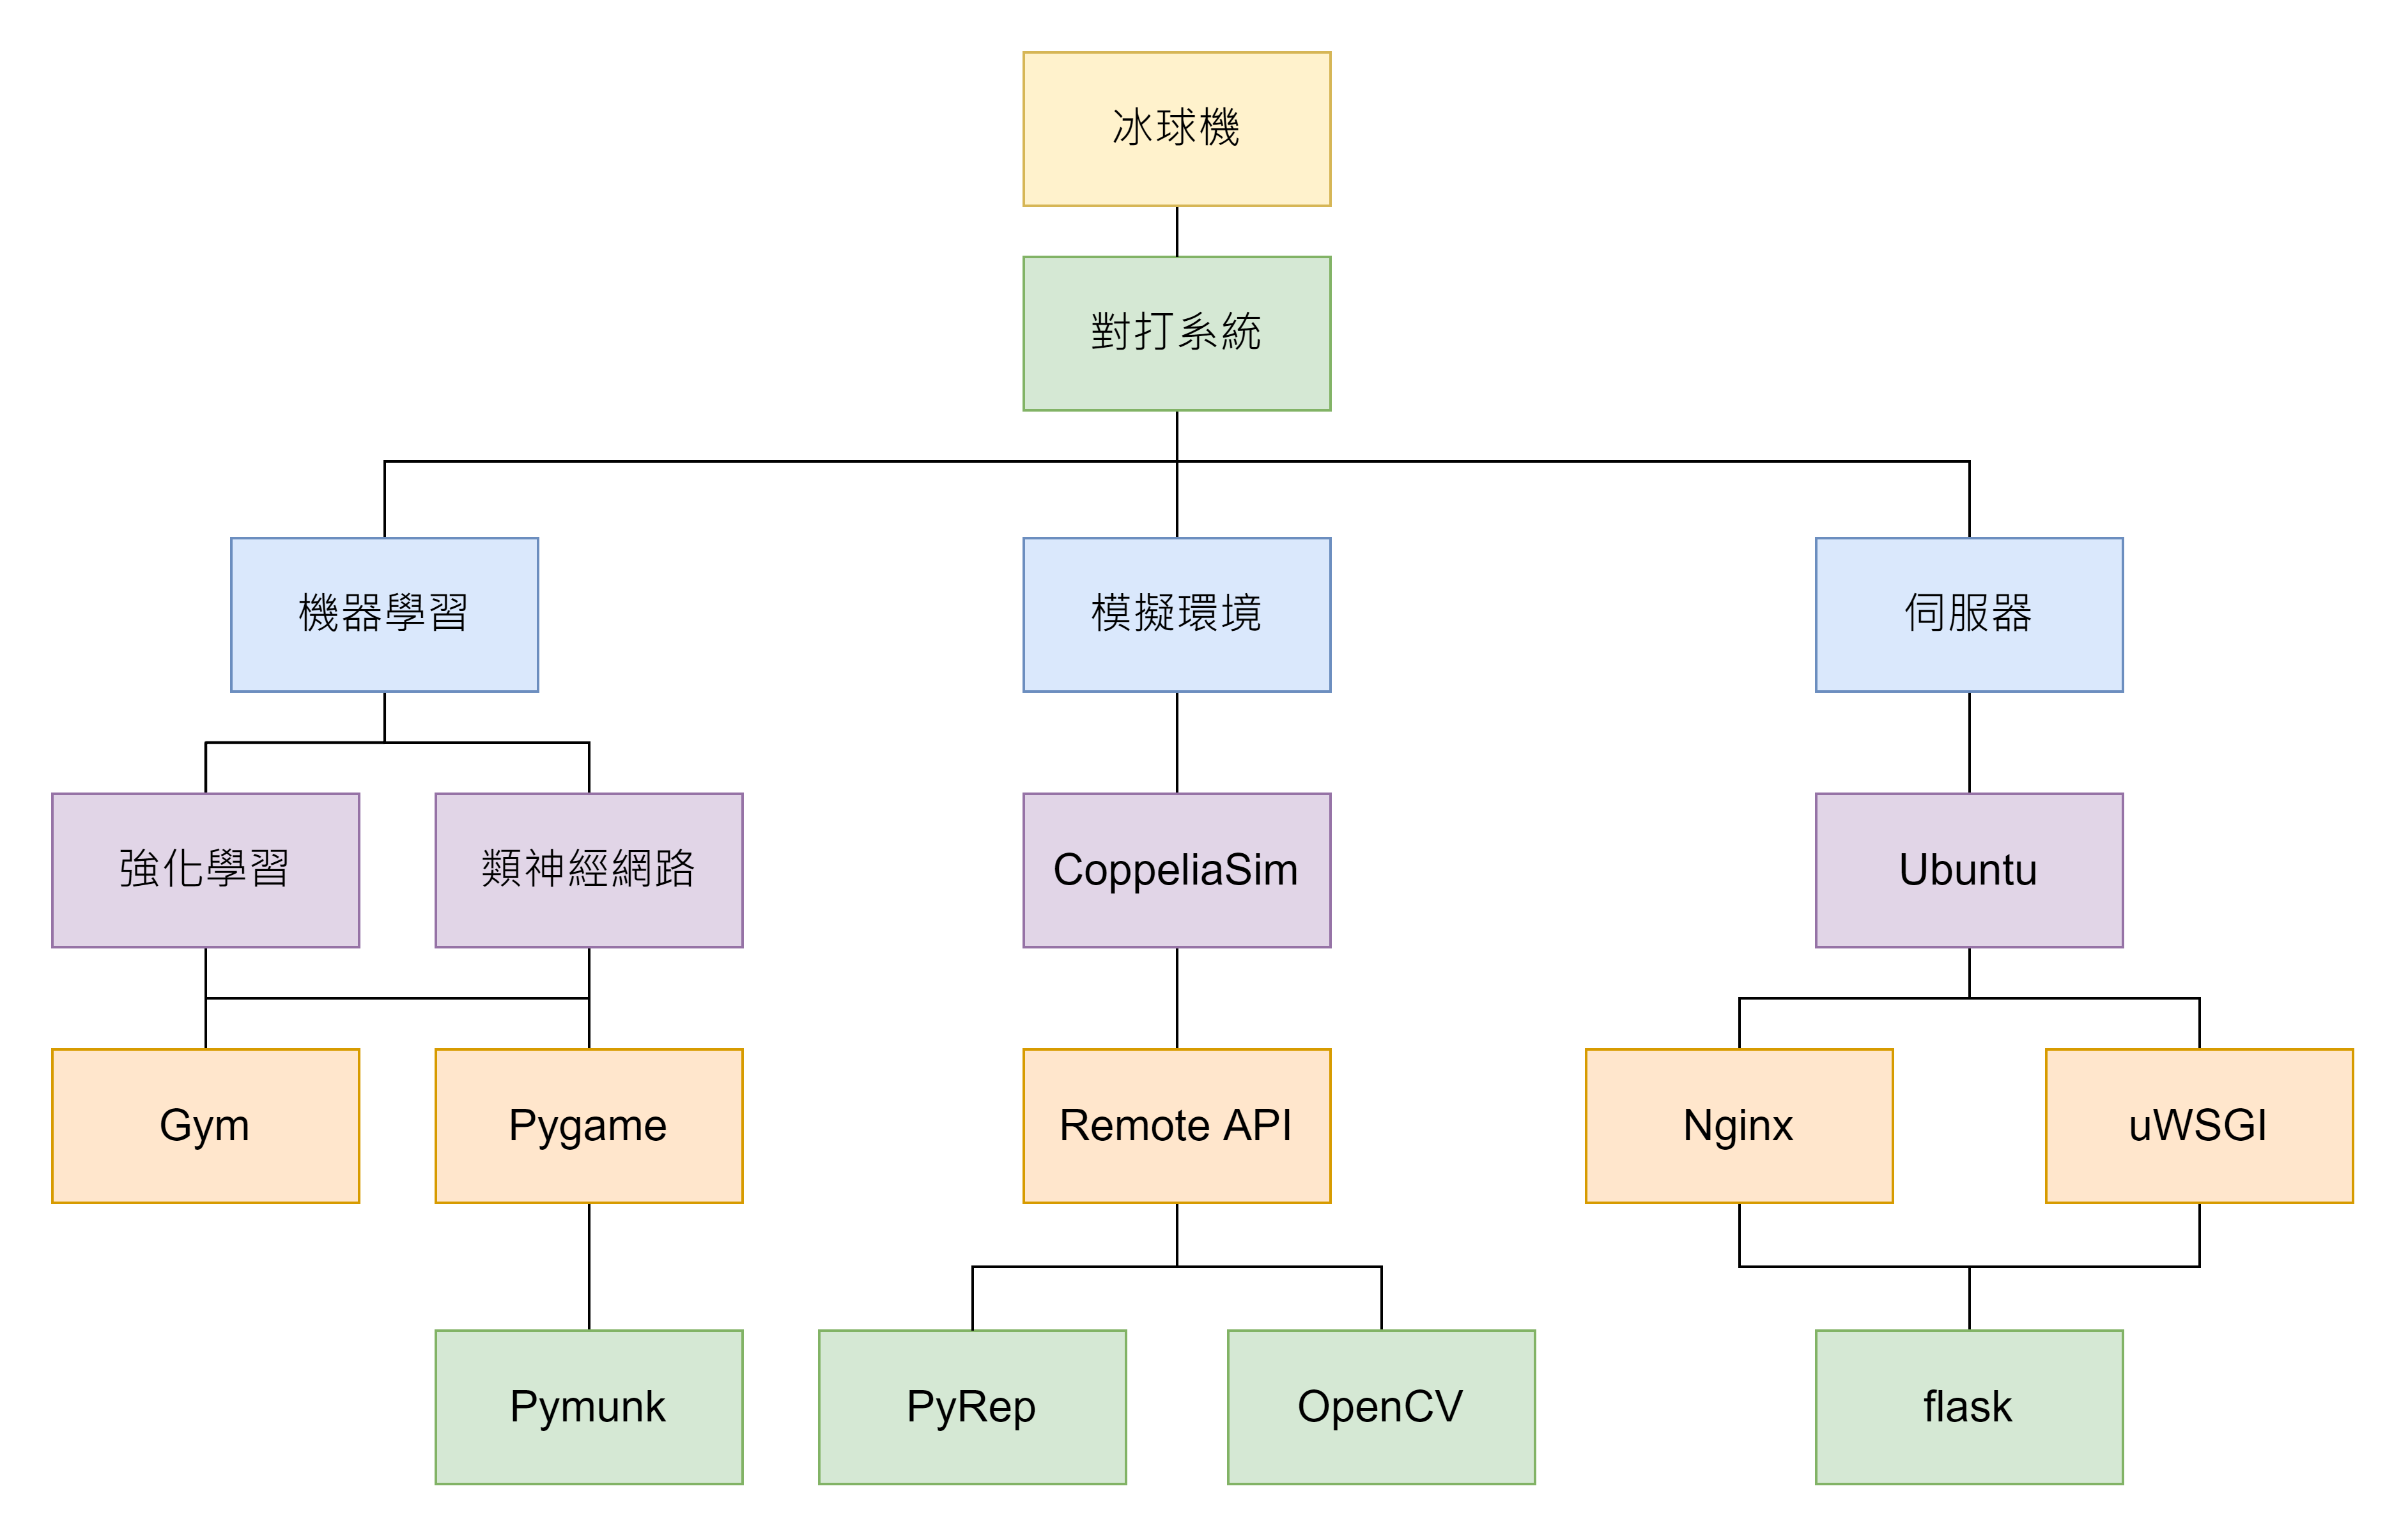
\includegraphics[width=15cm]{研究架構}
\caption{\Large 研究架構 }
\label{研究架構 }
\end{center}
\end{figure}
\section{未來展望}
此專題希望能利用現有完成的機械學習的算法,能發展成虛擬訓練,再將訓練完的機器學習應用到虛擬環境或是實體機電系統,並透過伺服器將影像串流提供玩家網頁介面進行遠端操控,同時提供多人觀看及時的比賽影像,將整個冰球機的控制和使用者間有更完善串聯,機電系統的部分達到最優化控制和虛實整合的應用。
\section{規則說明}
 Pong game 的遊戲規則簡單,透過擊錘將球打入對方球門即得一分,只要其中一方得21分就結束該局。擊錘只能沿單方向來回移動來進行防守和進攻。\\
遊戲規則如下:
\begin{enumerate}
\item 球打入敵方即得一分。
\item 擊錘只單一方向移動。
\item 最快贏得21分者獲勝,並結束該局遊戲。
\end{enumerate}

\renewcommand{\baselinestretch}{0.5} %設定行距



%=---------------附錄-----------------=%
\addcontentsline{toc}{chapter}{附錄} %新增目錄名稱

\newpage
%=-------------作者簡介-----------------=%
    \addcontentsline{toc}{chapter}{作者簡介}
    \begin{center}
	\fontsize{20pt}{0em}\selectfont \bf{作者簡介}\\
	\end{center}	
	{\begin{textblock}{6}(0,0.5)
	\begin{figure}
	
\includegraphics[width=1.25in]{member1}  %作者照片
	\end{figure}
	\end{textblock}}
	{\renewcommand\baselinestretch{0.99}\selectfont %設定以下行距
	{\begin{textblock}{15}(3.5,0.7)%{寬度}(以左上角為原點之右移量,下移量)
	\noindent\fontsize{14pt}{0em}\selectfont \makebox[4em][s]{姓名}\enspace:\enspace
    \fontsize{14pt}{0em}\selectfont \makebox[4em][s]{陳冠佑}\\     \hspace*{\fill} \\
    \fontsize{14pt}{0em}\selectfont \makebox[4em][s]{學號}\enspace:\enspace
    \fontsize{14pt}{0em}\selectfont \makebox[4em][s]{41023219} \\ %\makebox為文本盒子
    \hspace*{\fill} \\
    \fontsize{14pt}{0em}\selectfont \makebox[4em][s]{就讀學校}\enspace:\enspace
    \fontsize{14pt}{0em}\selectfont \makebox[9em][s]{國立虎尾科技大學}\\
    \fontsize{14pt}{0em}\selectfont \makebox[5em][s]{\quad}\enspace\enspace
    \fontsize{14pt}{0em}\selectfont \makebox[8em][s]{機械設計工程系}\\
    \hspace*{\fill} \\
    \fontsize{14pt}{0em}\selectfont \makebox[4em][s]{經歷}\enspace:\enspace
    \end{textblock}}}
   % \hspace*{\fill} \\
   \vspace{2em}
	{\begin{textblock}{6}(0,2.3)
	\begin{figure}
	
\includegraphics[width=1.15in]{member2}  %作者照片
    \end{figure}
    \end{textblock}}
    {\renewcommand\baselinestretch{0.99}
    \selectfont %設定以下行距
    {\begin{textblock}{15}(3.5,2.5) %{寬度}(以左上角為原點之右移量,下移量)
\noindent\fontsize{14pt}{0em}\selectfont \makebox[4em][s]{姓名}\enspace:\enspace
\fontsize{14pt}{0em}\selectfont \makebox[4em][s]{陳冠翰}\\ 
\hspace*{\fill} \\
\fontsize{14pt}{0em}\selectfont \makebox[4em][s]{學號}\enspace:\enspace
\noindent\fontsize{14pt}{0em}\selectfont \makebox[4em][s]{41023221} \\ 
\hspace*{\fill} \\
\fontsize{14pt}{0em}\selectfont \makebox[4em][s]{就讀學校}\enspace:\enspace
\fontsize{14pt}{0em}\selectfont \makebox[9em][s]{國立虎尾科技大學}\\
\fontsize{14pt}{0em}\selectfont \makebox[5em][s]{\quad}\enspace\enspace
\fontsize{14pt}{0em}\selectfont \makebox[8em][s]{機械設計工程系}\\
\hspace*{\fill} \\
\fontsize{14pt}{0em}\selectfont \makebox[4em][s]{經歷}\enspace:\enspace
    \end{textblock}}}
    %\hspace*{\fill} \\
    \vspace{2em}
    {\begin{textblock}{6}(0,4.1)
    \begin{figure}
        
\includegraphics[width=1.15in]{member3} %{}內是圖片文件的相對路徑
    \end{figure}
    \end{textblock}}
    {\renewcommand\baselinestretch{0.99}\selectfont %設定以下行距
    {\begin{textblock}{15}(3.5,4.3) %{寬度}(以左上角為原點之右移量,下移量)
\noindent\fontsize{14pt}{0em}\selectfont \makebox[4em][s]{姓名}\enspace:\enspace%\noindent指定首行不進行縮排
\fontsize{14pt}{0em}\selectfont \makebox[4em][s]{陳奕倫}\\ 
\hspace*{\fill} \\
\noindent\fontsize{14pt}{0em}\selectfont \makebox[4em][s]{學號}\enspace:\enspace
\noindent\fontsize{14pt}{0em}\selectfont \makebox[4em][s]{41023222} \\ %\makebox為文本盒子
\hspace*{\fill} \\
\noindent\fontsize{14pt}{0em}\selectfont \makebox[4em][s]{就讀學校}\enspace:\enspace
\noindent\fontsize{14pt}{0em}\selectfont \makebox[9em][s]{國立虎尾科技大學}\\
\noindent\fontsize{14pt}{0em}\selectfont \makebox[5em][s]{\quad}\enspace\enspace
\noindent\fontsize{14pt}{0em}\selectfont \makebox[8em][s]{機械設計工程系}\\
\hspace*{\fill} \\
\noindent\fontsize{14pt}{0em}\selectfont \makebox[4em][s]{經歷}\enspace:\enspace
    \end{textblock}}}
   % \hspace*{\fill} \\
   \vspace{2em}
    {\begin{textblock}{6}(0,5.9)
    \begin{figure}
        
\includegraphics[width=1.15in]{member4} %{}內是圖片文件的相對路徑
    \end{figure}
    \end{textblock}}
    {\renewcommand\baselinestretch{0.99}\selectfont %設定以下行距
    {\begin{textblock}{15}(3.5,6.1) %{寬度}(以左上角為原點之右移量,下移量)
\noindent\noindent\fontsize{14pt}{0em}\selectfont \makebox[4em][s]{姓名}\enspace:\enspace
\noindent\fontsize{14pt}{0em}\selectfont \makebox[4em][s]{陳瑨維}\\ \hspace*{\fill} \\
\noindent\fontsize{14pt}{0em}\selectfont \makebox[4em][s]{學號}\enspace:\enspace
\noindent\fontsize{14pt}{0em}\selectfont \makebox[4em][s]{41023228} \\ \hspace*{\fill} \\
\noindent\fontsize{14pt}{0em}\selectfont \makebox[4em][s]{就讀學校}\enspace:\enspace
\noindent\fontsize{14pt}{0em}\selectfont \makebox[9em][s]{國立虎尾科技大學}\\
\noindent\fontsize{14pt}{0em}\selectfont \makebox[5em][s]{\quad}\enspace\enspace
\noindent\fontsize{14pt}{0em}\selectfont \makebox[8em][s]{機械設計工程系}\\
\hspace*{\fill} \\
\noindent\fontsize{14pt}{0em}\selectfont \makebox[4em][s]{經歷}\enspace:\enspace
    \end{textblock}}}
    %\hspace*{\fill} \\
\vspace{2em}
    {\begin{textblock}{6}(0,7.7)
    \begin{figure}
        
\includegraphics[width=1.15in]{member5} %{}內是圖片文件的相對路徑
    \end{figure}
    \end{textblock}}
    
\newpage
%=----------------書背----------------------=%
\pagestyle{empty}%設定沒有頁眉和頁腳
\begin{center}
\fontsize{0.001pt}{1pt}\selectfont .\\
\vspace{4em}
\fontsize{30pt}{30pt}\selectfont 【13】 \\
\fontsize{20pt}{20pt}\selectfont
\vspace{0.5em}
分\\
類\\
編\\
號\\
\vspace{0.5em}
\hspace{-0.5em}:\\
\vspace{0.5em}
\rotatebox[origin=cc]{270}{\sectionef\LARGE \textbf{112-4-APP-3004-1}}\\ %旋轉
\vspace{0.5em}
網\\
際\\

足\\
球\\
場\\
景\\
設\\
計\\
\vspace{2em}
一\\
一\\
二\\
級\\

\end{center}
%\newpage
%\begin{landscape}  %橫式環境
%\begin{center}
%\fontsize{0.001pt}{1pt}\selectfont .
%\vspace{70mm}
%\rotatebox[origin=cc]{90}{\LARGE 【14】}\rotatebox[origin=cc]%{180}{\LARGE 1-2-APP-8765} %旋轉
%\end{center}
%\end{landscape}
\end{document}
